\documentclass[14pt]
{article}

%basiques
\usepackage[utf8x]{inputenc}
\usepackage[T1]{fontenc}
\usepackage[french]{babel}

%math
\usepackage{amsmath}
\usepackage{amssymb}

% images
\usepackage{graphicx}

%mise en page
\usepackage{fancyhdr}
\usepackage{fancybox}
\usepackage{geometry}

\newcommand\tab[1][1cm]{\hspace*{#1}}

\geometry{hmargin=4cm}

\begin{document}
% Entete
\pagestyle{fancy}
\lhead{Léa Heiniger}
\rhead{04.10.2021}
\chead{\textbf{Data science}}

\begin{center}
	\section*{\textbf{{\LARGE TP1 : Linear Algebra}}}
\end{center}
\bigskip\bigskip\bigskip

\section{Matrix} % 1
\bigskip
\paragraph*{1.} We want to find a quadratic function $f(x)=ax^{2}+bx+c$ such that $f(1)=1$, $f(2)=9$ and $f(3)=27$. To find $a$, $b$ and $c$ we we solve the following system of equations :\\
$\begin{cases}a+b+c=1\\4a+2b+c=9\\9a+3b+c=27\end{cases} \Leftrightarrow \begin{cases}a+b+c=1\\6b+5c=-27\\9a+3b+c=27\end{cases} \Leftrightarrow \begin{cases}3b+4c=-9\\6b+5c=-27\\9a+3b+c=27\end{cases} \Leftrightarrow \begin{cases}c=3\\6b+5c=-27\\9a+3b+c=27\end{cases} \Leftrightarrow \begin{cases}c=3\\b=-7\\9a+3b+c=27\end{cases} \Leftrightarrow \begin{cases}c=3\\b=-7\\a=5\end{cases}$\\
The quadratic function is $f(x)=5x^{2}-7x+3$\\

\paragraph*{2.} We solve the system of linear equations for $x$ and $y$ :\\
$\begin{cases}x+ay=2\\bx+2y=3\end{cases} \Leftrightarrow \begin{cases}bx+bay=2b\\bx+2y=3\end{cases} \Leftrightarrow \begin{cases}(ba-2)y=2b-3\\bx+2y=3\end{cases} \Leftrightarrow \begin{cases}y=\frac{2b-3}{ba-2}\\bx+2\frac{2b-3}{ba-2}=3\end{cases} \Leftrightarrow \begin{cases}y=\frac{2b-3}{ba-2}\\x=\frac{3-2\frac{2b-3}{ba-2}}{b}\end{cases}$

\section{The importance of the mathematical concept behind a
code} % 2
\bigskip
\paragraph*{1.} The function \texttt{project\_on\_first(u,v)} takes two column vectors $\mathbf{u}$ and $\mathbf{v}$ and it returns the projection of $\mathbf{v}$ over $\mathbf{u}$. the projection $\mathbf{v'}$ and $\mathbf{u}$ are collinear ($\exists\ \alpha$, $\mathbf{v'}*\alpha = \mathbf{u}$)\\
\begin{figure}[h]
\centering
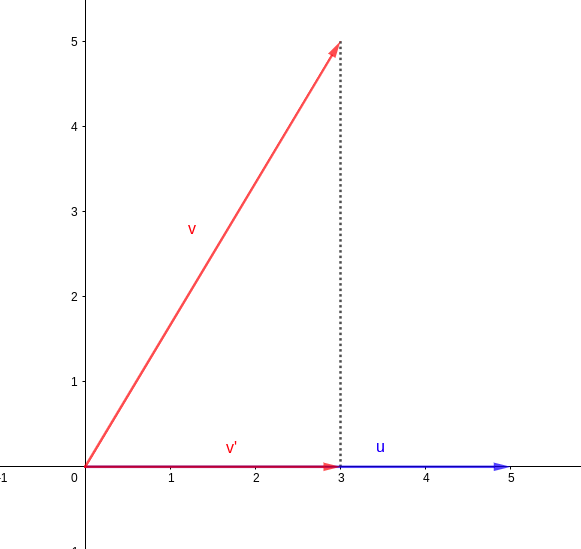
\includegraphics[scale=0.3]{ab.png}
\end{figure}

\paragraph*{2.} The last lines of the program perform a scalar product between the two vectors $u$ and $v$ (taking two vectors and returns a scalar) $\mathbf{u}\cdot \mathbf{v}=\displaystyle\sum_{i} u_{i}v_{i}$ The \texttt{zip()} function takes two lists of same size and creates a list of tuples with the values of the two lists. The last line multiply the two values of each tuples and sum all these products (which corresponds indeed to the formula of the scalar product)\\
We can rewrite those three line as \texttt{r=np.dot(u,v)} (using the numpy library)\\

%\paragraph*{3.} Code in the file \texttt{some\_script.py}, I created the function \texttt{orthogonal(u)}

\section{Computing Eigenvalues, Eigenvectors, and Determinants} % 3
\bigskip
\paragraph*{1.}We compute the determinant, the eigenvectors and the eigenvalues of the matrix $A=\begin{bmatrix}
1 & 1 & 3 \\ 
1 & 5 & 1 \\ 
3 & 1 & 1
\end{bmatrix} $. \\
\\
determinant : $det(A)=1\times(5\times1-1\times1)+(-1)\times(1\times1-1\times3)+3\times(1\times1-5\times3) =4+2-42=-36$ \\
\\
eigenvalues : $det(A - I\lambda)= 0 <=> det\left( \begin{matrix} (1 - \lambda) & 1 & 3 \\ 1 & (5 - \lambda) & 1 \\ 3 & 1 & (1 - \lambda) \end{matrix} \right) = 0= (1 - \lambda) \times (4 - 6\lambda + \lambda^{2}) - 1 \times (2 + \lambda) + 3 \times (1 - 15 + 3\lambda) = -36 + 7\lambda^{2} - \lambda^{3} = -(\lambda + 2)(\lambda - 3)(\lambda - 6)$\\
The eigenvalues are $\{-2, 3, 6\}$\\
eigenvectors : We solve $(A-\lambda I)\mathbf{v}=\mathbf{0}$ for each possible $\lambda$ to fin the eigenvectors and we find :\\
$\mathbf{v}=(-1,0,1)$ for $\lambda =-2$, $\mathbf{v}=(1,-1,1)$ for $\lambda =3$ and $\mathbf{v}=(1,2,1)$ for $\lambda =6$
%\paragraph*{2.}
\paragraph*{3.} The code can be found in the file \texttt{ex3.py}

\section{Computing Projection Onto a Line} % 4
\bigskip
\paragraph*{1.} We want to find the distance between $A(5, 4)$ and the line $\alpha : 3x - 2y = -6$. We start by rewriting $\alpha$ as the function $\alpha (x)=\frac{-6 +2y}{3}$. Then we pick two values $x_{1}$ and $x_{2}$ and compute $\alpha (x_{1}=y_{1})$ and $\alpha (x_{2}=y_{2})$. We compute a vector $\mathbf{u}$ collinear to $\alpha$: $\mathbf{u} = \begin{bmatrix} x_{2} - x_{1}\\y_{2} - y_{1} \end{bmatrix}$. Then we compute $\mathbf{v}$, a vector between a point of $\alpha$ and $A$ : $\mathbf{v} = \begin{bmatrix} x_{1} - A_{x}\\y_{1} - A_{y} \end{bmatrix}$. We compute two vectors, $\mathbf{w_{1}}$ the projection of $\mathbf{v}$ over $\mathbf{u}$ and $\mathbf{w_{2}} = \mathbf{v}-\mathbf{w_{1}}$. Since $\mathbf{w_{2}}$ is collinear to $\mathbf{u}$, $||\mathbf{w_{2}}||$, corresponds to the distance between $A$ and $\alpha$.
%\paragraph*{2.}

\end{document}